\documentclass[fleqn,11pt]{article}

\usepackage[letterpaper,margin=0.75in]{geometry}

\usepackage{amsmath}
\usepackage{booktabs}
\usepackage{graphicx}
\usepackage{listings}

\setlength{\parindent}{1.4em}

\begin{document}

\lstset{
  language=Python,
  basicstyle=\small,          % print whole listing small
  keywordstyle=\bfseries,
  identifierstyle=,           % nothing happens
  commentstyle=,              % white comments
  stringstyle=\ttfamily,      % typewriter type for strings
  showstringspaces=false,     % no special string spaces
  numbers=left,
  numberstyle=\tiny,
  numbersep=5pt,
  frame=tb,
}

\title{Congestion Control}

\author{Devon Kinghorn}

\date{}

\maketitle

\section{TCP Tahoe}

TCP Tahoe is an early implementation of TCP. It is very simple and robust. 
TCP Tahoe maxamizes bandwidth usage by trying to keep a full queue. 
To fill up a queue without losing packets Tahoe has a few simple rules.

\begin{enumerate}
  \item Setting an initial slow start threshold. 
  This will be used to quickly increase bandwidth.
  \item Slow Start. Slow Start is very simple. 
  Whenever an ACK is received and the current window size ($CWND$) is less than the threshold, increase the window size by the number of packets received.
  \item Additive Increase. Whenever an ACK is received and the window size is greater than the threshold, the window size is increased by 
  $\frac{MSS * B}{CWND}$.
   Where $MSS$ is the Maximum Segment Size and $B$ is the number of bytes acked.
   \item When a loss event is detected by either a timeout or 3 duplicate ACKs, set $CWND$ to $1 * MSS$ 
   and the threshold to $max(\frac{CWND}{2},MSS)$
   \item Ensure that $CWND$ is a multiple of $MSS$ by using an increment variable. In a loss event reset increment to zero.
\end{enumerate}

When a loss event is triggered, it generally means that the router buffers overflowed and that the 
sender was sending packets too quickly.
By lowering the threshold, it means that the sender will get to half of the rate that overflowed the buffer quickly with slow start then use additive increase to slowly increase the bandwidth used by the sender.
This maxamizes the time that the sender spends sending packets close to the max bandwidth of the connection to the receiver.


\section{Experiments}

In this report I set up a simple network with the following configuration
\begin{lstlisting}[title={Network Configuration for Experiments}]
# n1 -- n2
#
n1 n2
n2 n1

# link configuration
n1 n2 1Mbps 100ms
n2 n1 1Mbps 100ms
\end{lstlisting}
The network was used in every experiment in this report. 
The initial $threshold$ for every experiment was 100,000 bytes, and the $MSS$ was always 1000 bytes
Every experiment was performed sending the file $internet-architecture.pdf$ from $n1$ to $n2$


\subsection{Slow Start}

To show how slow start works, I sent the file $internet-architecture.pdf$ without any loss.
Below is a graph of the size of the congestion window relative to time.

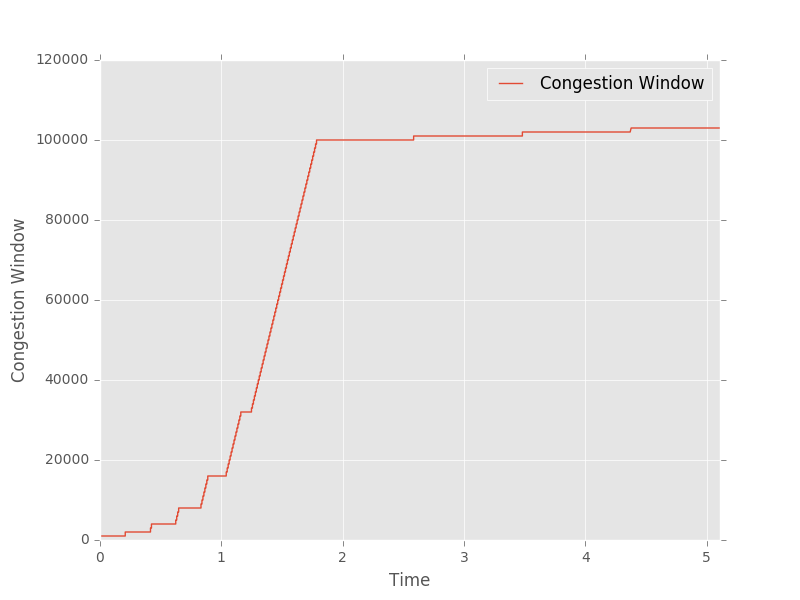
\includegraphics[width=11cm]{graphs/cwndbasic.png}

Slow start ensures that the window size quickly grows up until the threshold is met. 
At this point the window size grows very slowly. It is noteable that the window increases in size by 1 $MSS$ less frequently than the initial round trip time.
This is because the network has a large queue of packets. 
As $n1$ increases the rate at which it sends out packets, the window size increases but so does the round trip time so the bandwidth never exceeds 1Mbps.

Although it looks like the window size increases by more than 1000 bytes, that is just because the node receives AKCs in short bursts.
The window size never increases any amount other than 1000 bytes.

\subsection{One Packet Loss}

To show how TCP Tahoe handles a single packet loss I set the network to lose packet with byte 14000 (packet number 14). 

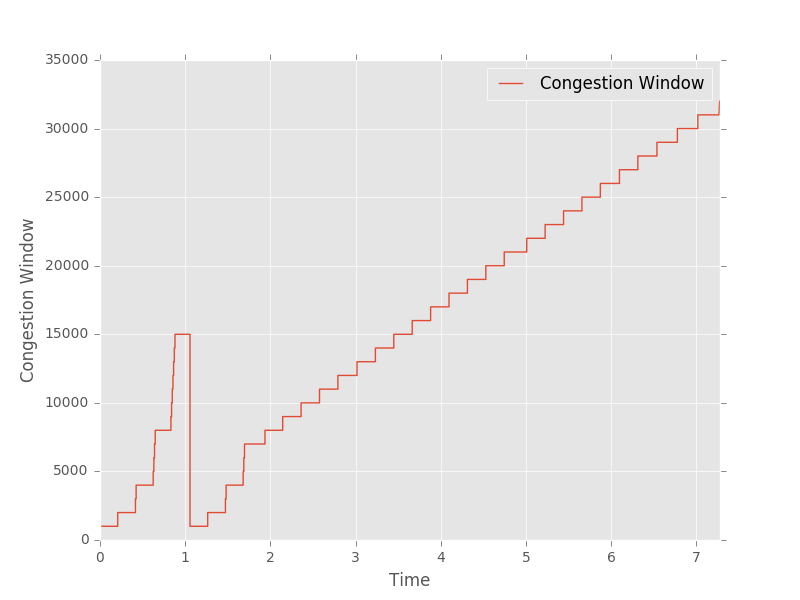
\includegraphics[width=11cm]{graphs/cwnd14.png}

The packet was lost at about one second. 
At this point the window size dropped to zero. 
The threshold was set to 7000 and that can be seen from slow start stopping around 1.8 seconds.
Additive increase then controls the rate at which the window increases.

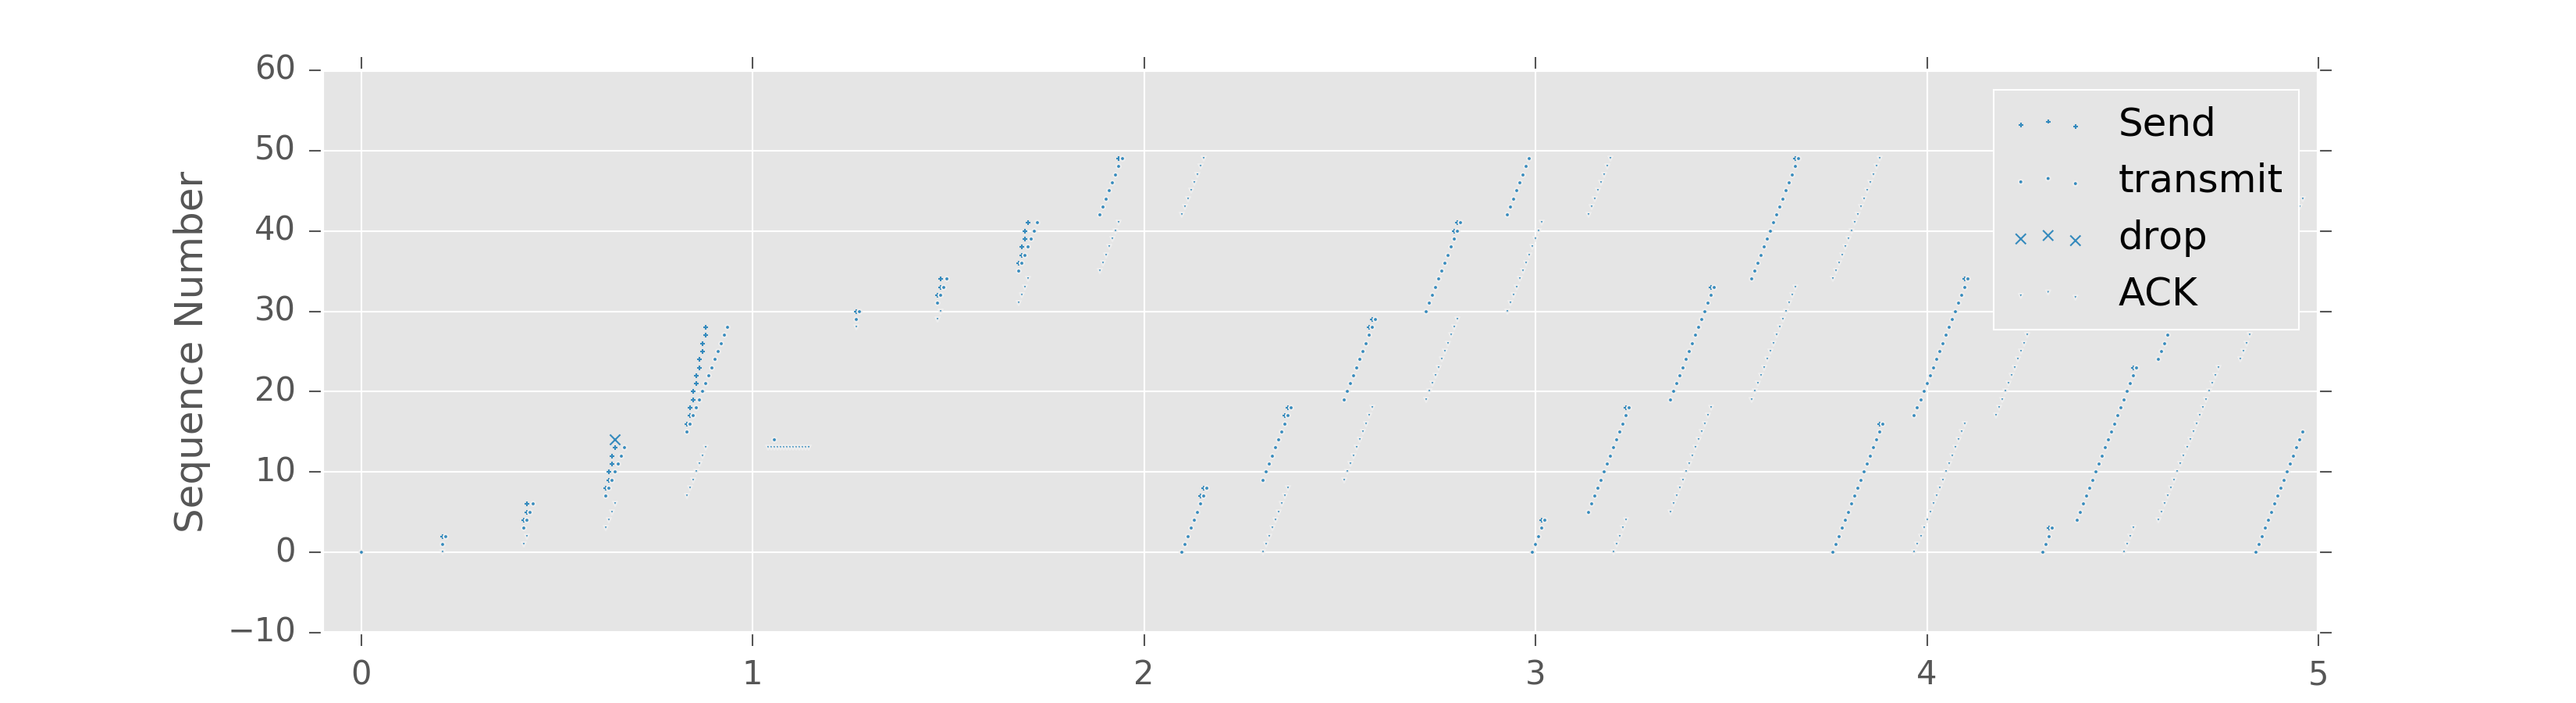
\includegraphics[width=16cm]{graphs/sequence14.png}

Above is a sequence graph for the experiment. After packet 14 is lost, packets 15-28 are still sent.
Once the third duplicate ACK from receiving packet 13 arrive the loss event was triggered and packet 14 was sent again.
The receiver had received all of the packets through 28 so once packet 14 was received an ACK for 29 was received.
From there slow start increases until the threshold is reached. 

\subsection{Two Packet Loss}

When a packet is lost, the sender forgets about all sent packets. 
This brings up challenges when sending packets. Which have been lost and which arrived.
To visualize how TCP Tahoe handles two lost packets, I made the network lose packet 14 and packet 28.

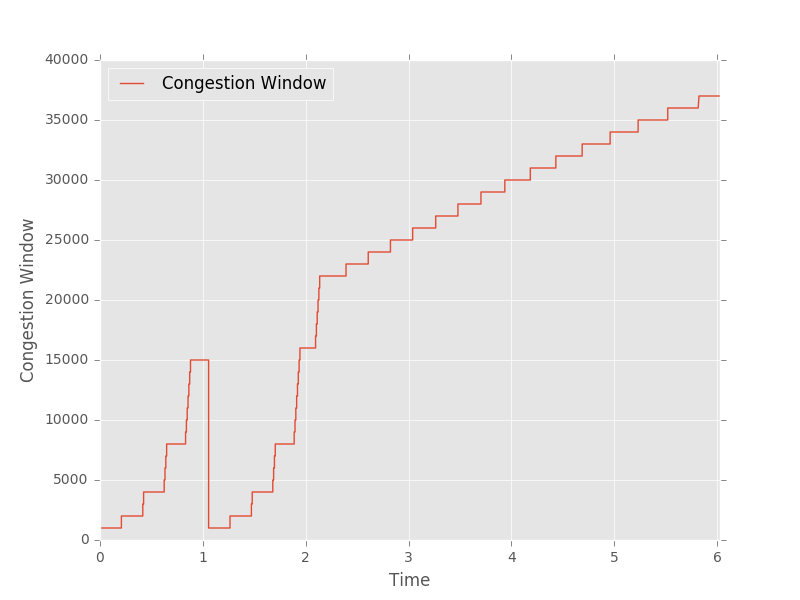
\includegraphics[width=11cm]{graphs/cwnd1428.png}

Even though two packets were lost the window size is identical to when one packet was lost.
This is because the state was lost so the sender didn't know if it sent 27 or 28 last.
The node just received an ACK from the receiver acknowledging packet 27 had arrived as opposed to 28 in the previous experiment. 

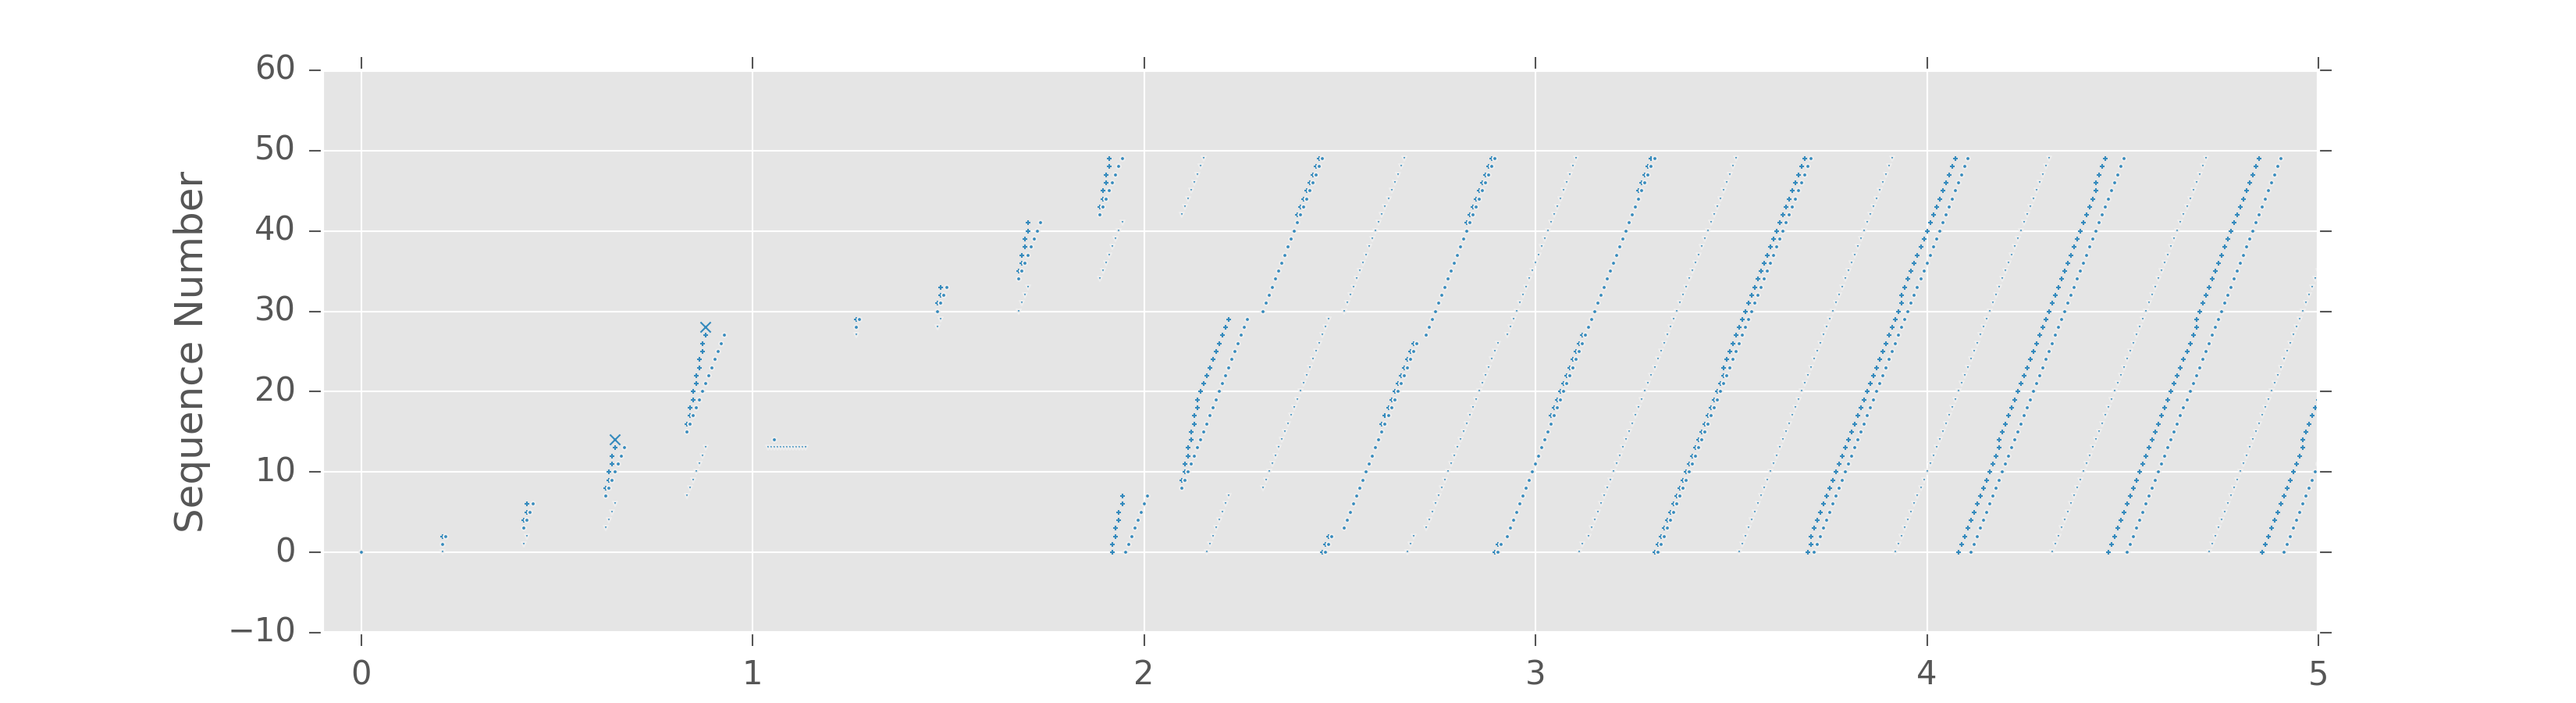
\includegraphics[width=16cm]{graphs/sequence1428.png}

The Sequence graph looks nearly identical to the single loss packet experiment. 
The only difference is that slow start begin by sending packet 28 instead of 29. 
Losing three packets proves to be the most interesting.

\subsection{Three Packet Loss}

Losing three packets in a window throws off TCP Reno. 
It remembers that some packets were sent and assumes that other packets were received.
This assumption causes it to pause until a timeout is triggered then slow start begins.
TCP Tahoe remembers no state and this experiment shows how not storing state is advantageous sometimes.
For this experiment, I sent the file with the packets 14,26, and 28 all lost on the first attempt.

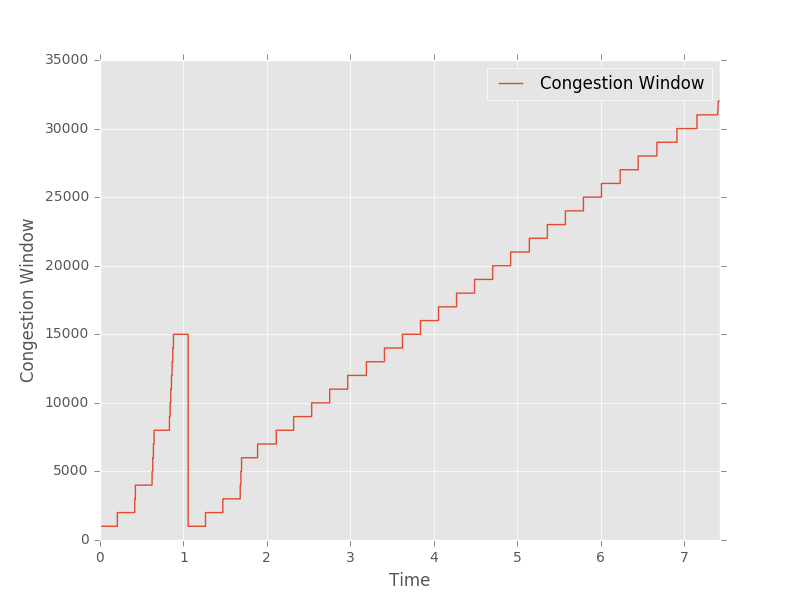
\includegraphics[width=11cm]{graphs/cwnd142628.png}

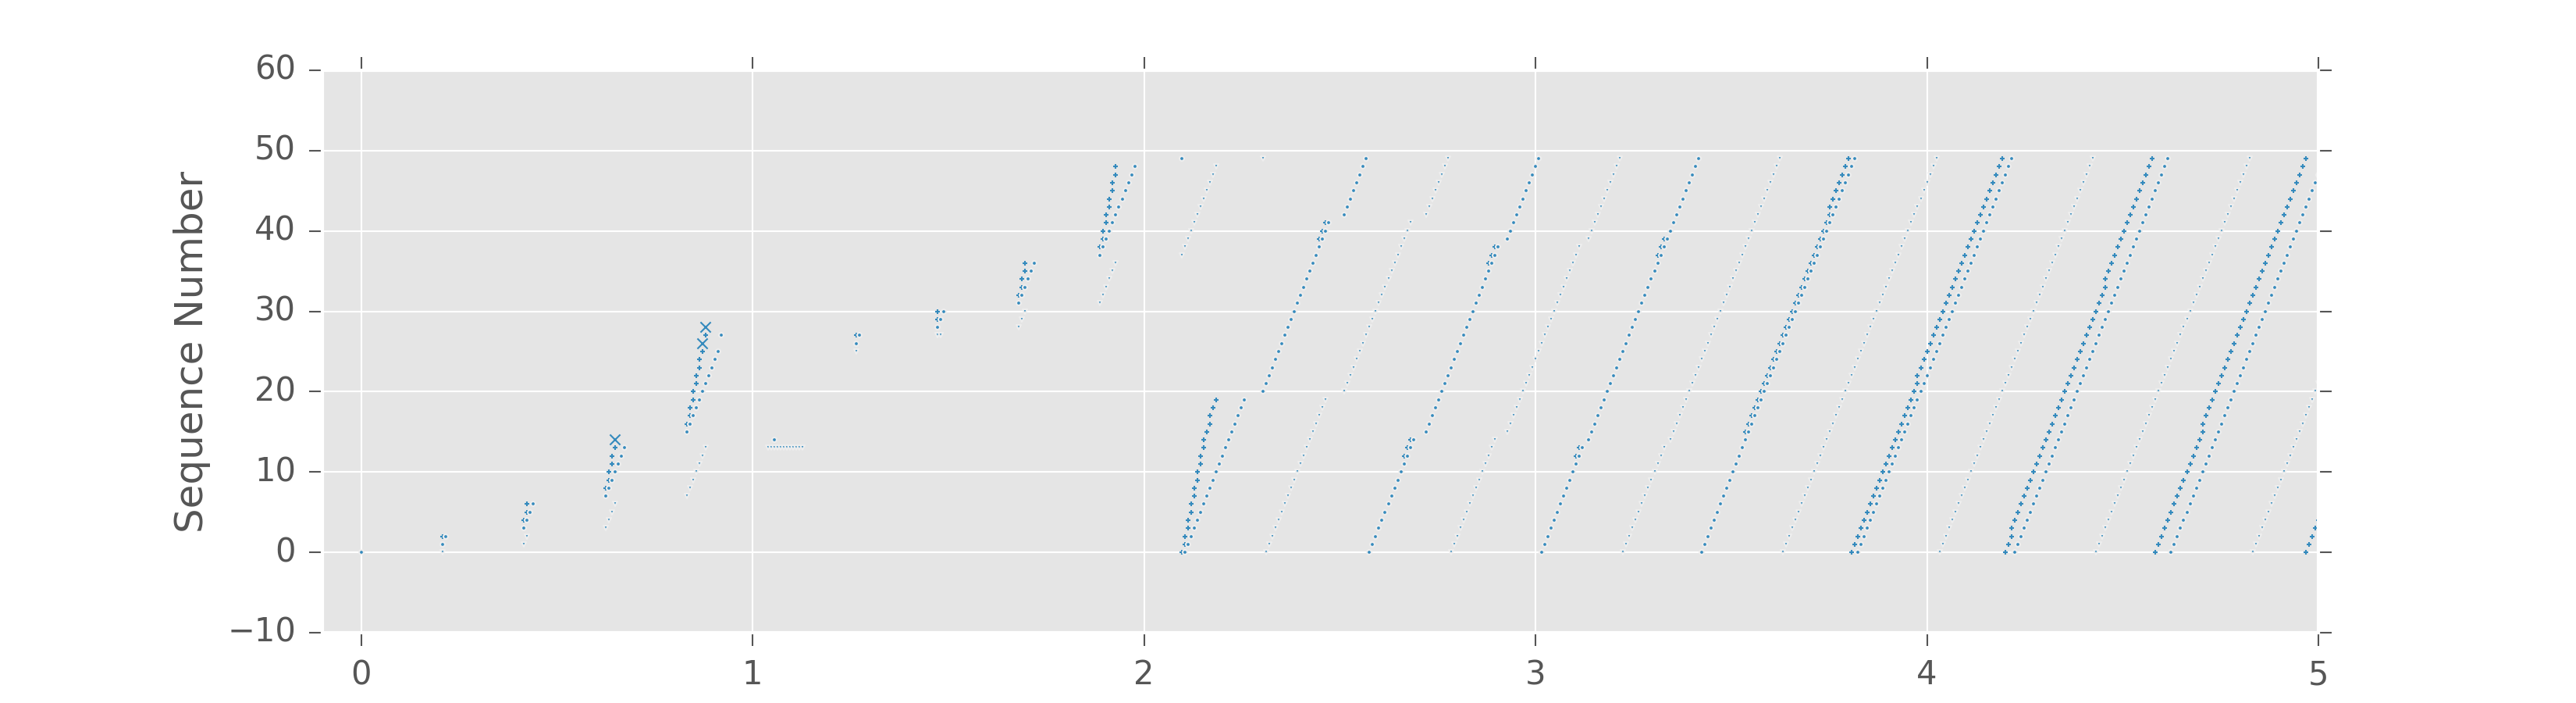
\includegraphics[width=16cm]{graphs/sequence142628.png}

TCP Tahoe shines when other algorithms make flawed assumptions. 
It is very simple and it shows in the graphs above. 
When packet 14 is sent again, the $n1$ receives an ack to resend packet 26. So $n1$ sends 26 and 27.
At this point the transmission of the file resumes as normal sending 28-31.
It is true that packet 27 was sent when it didn't need to be, but the amount of bandwidth wasted is minimal.


\section{Conclusion}

TCP Tahoe is a very simple implementation of TCP. 
It handles loss events very well because it remembers no state after a retransmit event.
This does cause the problem that packets can be unnecessarily sent again as seen in the experiment with three lost packets,
but the assumption that all packets were lost creates a very robust implementation of TCP.


\end{document}